\documentclass{ximera}

%\usepackage{todonotes}

\newcommand{\todo}{}

\usepackage{tkz-euclide}
\tikzset{>=stealth} %% cool arrow head
\tikzset{shorten <>/.style={ shorten >=#1, shorten <=#1 } } %% allows shorter vectors

\usepackage{tkz-tab}  %% sign charts
\usetikzlibrary{decorations.pathreplacing} 

\usetikzlibrary{backgrounds} %% for boxes around graphs
\usetikzlibrary{shapes,positioning}  %% Clouds and stars
\usetikzlibrary{matrix} %% for matrix
\usepgfplotslibrary{polar} %% for polar plots
\usetkzobj{all}
\usepackage[makeroom]{cancel} %% for strike outs
%\usepackage{mathtools} %% for pretty underbrace % Breaks Ximera
\usepackage{multicol}

\usepackage{polynom}



\usepackage[many]{tcolorbox}  %% for titled boxes
\newtcolorbox{xbox}[1]{%
    tikznode boxed title,
    enhanced,
    arc=0mm,
    interior style={white},
    attach boxed title to top center= {yshift=-\tcboxedtitleheight/2},
    fonttitle=\bfseries,
    colbacktitle=white,coltitle=black,
    boxed title style={size=normal,colframe=white,boxrule=0pt},
    title={#1}}


\usepackage{array}
\setlength{\extrarowheight}{+.1cm}   
\newdimen\digitwidth
\settowidth\digitwidth{9}
\def\divrule#1#2{
\noalign{\moveright#1\digitwidth
\vbox{\hrule width#2\digitwidth}}}





\newcommand{\RR}{\mathbb R}
\newcommand{\R}{\mathbb R}
\newcommand{\N}{\mathbb N}
\newcommand{\Z}{\mathbb Z}

%\renewcommand{\d}{\,d\!}
\renewcommand{\d}{\mathop{}\!d}
\newcommand{\dd}[2][]{\frac{\d #1}{\d #2}}
\newcommand{\pp}[2][]{\frac{\partial #1}{\partial #2}}
\renewcommand{\l}{\ell}
\newcommand{\ddx}{\frac{d}{\d x}}
\newcommand{\ddt}{\frac{d}{\d t}}

\newcommand{\zeroOverZero}{\ensuremath{\boldsymbol{\tfrac{0}{0}}}}
\newcommand{\inftyOverInfty}{\ensuremath{\boldsymbol{\tfrac{\infty}{\infty}}}}
\newcommand{\zeroOverInfty}{\ensuremath{\boldsymbol{\tfrac{0}{\infty}}}}
\newcommand{\zeroTimesInfty}{\ensuremath{\small\boldsymbol{0\cdot \infty}}}
\newcommand{\inftyMinusInfty}{\ensuremath{\small\boldsymbol{\infty - \infty}}}
\newcommand{\oneToInfty}{\ensuremath{\boldsymbol{1^\infty}}}
\newcommand{\zeroToZero}{\ensuremath{\boldsymbol{0^0}}}
\newcommand{\inftyToZero}{\ensuremath{\boldsymbol{\infty^0}}}



\newcommand{\numOverZero}{\ensuremath{\boldsymbol{\tfrac{\#}{0}}}}
\newcommand{\dfn}{\textbf}
%\newcommand{\unit}{\,\mathrm}
\newcommand{\unit}{\mathop{}\!\mathrm}
\newcommand{\eval}[1]{\bigg[ #1 \bigg]}
\newcommand{\seq}[1]{\left( #1 \right)}
\renewcommand{\epsilon}{\varepsilon}
\renewcommand{\iff}{\Leftrightarrow}

\DeclareMathOperator{\arccot}{arccot}
\DeclareMathOperator{\arcsec}{arcsec}
\DeclareMathOperator{\arccsc}{arccsc}
\DeclareMathOperator{\si}{Si}
\DeclareMathOperator{\proj}{proj}
\DeclareMathOperator{\scal}{scal}


\newcommand{\tightoverset}[2]{% for arrow vec
  \mathop{#2}\limits^{\vbox to -.5ex{\kern-0.75ex\hbox{$#1$}\vss}}}
\newcommand{\arrowvec}[1]{\tightoverset{\scriptstyle\rightharpoonup}{#1}}
\renewcommand{\vec}{\mathbf}
\newcommand{\veci}{\vec{i}}
\newcommand{\vecj}{\vec{j}}
\newcommand{\veck}{\vec{k}}
\newcommand{\vecl}{\boldsymbol{\l}}

\newcommand{\dotp}{\bullet}
\newcommand{\cross}{\boldsymbol\times}
\newcommand{\grad}{\boldsymbol\nabla}
\newcommand{\divergence}{\grad\dotp}
\newcommand{\curl}{\grad\cross}
%\DeclareMathOperator{\divergence}{divergence}
%\DeclareMathOperator{\curl}[1]{\grad\cross #1}


\colorlet{textColor}{black} 
\colorlet{background}{white}
\colorlet{penColor}{blue!50!black} % Color of a curve in a plot
\colorlet{penColor2}{red!50!black}% Color of a curve in a plot
\colorlet{penColor3}{red!50!blue} % Color of a curve in a plot
\colorlet{penColor4}{green!50!black} % Color of a curve in a plot
\colorlet{penColor5}{orange!80!black} % Color of a curve in a plot
\colorlet{fill1}{penColor!20} % Color of fill in a plot
\colorlet{fill2}{penColor2!20} % Color of fill in a plot
\colorlet{fillp}{fill1} % Color of positive area
\colorlet{filln}{penColor2!20} % Color of negative area
\colorlet{fill3}{penColor3!20} % Fill
\colorlet{fill4}{penColor4!20} % Fill
\colorlet{fill5}{penColor5!20} % Fill
\colorlet{gridColor}{gray!50} % Color of grid in a plot

\newcommand{\surfaceColor}{violet}
\newcommand{\surfaceColorTwo}{redyellow}
\newcommand{\sliceColor}{greenyellow}




\pgfmathdeclarefunction{gauss}{2}{% gives gaussian
  \pgfmathparse{1/(#2*sqrt(2*pi))*exp(-((x-#1)^2)/(2*#2^2))}%
}


%%%%%%%%%%%%%
%% Vectors
%%%%%%%%%%%%%

%% Simple horiz vectors
\renewcommand{\vector}[1]{\left\langle #1\right\rangle}


%% %% Complex Horiz Vectors with angle brackets
%% \makeatletter
%% \renewcommand{\vector}[2][ , ]{\left\langle%
%%   \def\nextitem{\def\nextitem{#1}}%
%%   \@for \el:=#2\do{\nextitem\el}\right\rangle%
%% }
%% \makeatother

%% %% Vertical Vectors
%% \def\vector#1{\begin{bmatrix}\vecListA#1,,\end{bmatrix}}
%% \def\vecListA#1,{\if,#1,\else #1\cr \expandafter \vecListA \fi}

%%%%%%%%%%%%%
%% End of vectors
%%%%%%%%%%%%%

%\newcommand{\fullwidth}{}
%\newcommand{\normalwidth}{}



%% makes a snazzy t-chart for evaluating functions
%\newenvironment{tchart}{\rowcolors{2}{}{background!90!textColor}\array}{\endarray}

%%This is to help with formatting on future title pages.
\newenvironment{sectionOutcomes}{}{} 



%% Flowchart stuff
%\tikzstyle{startstop} = [rectangle, rounded corners, minimum width=3cm, minimum height=1cm,text centered, draw=black]
%\tikzstyle{question} = [rectangle, minimum width=3cm, minimum height=1cm, text centered, draw=black]
%\tikzstyle{decision} = [trapezium, trapezium left angle=70, trapezium right angle=110, minimum width=3cm, minimum height=1cm, text centered, draw=black]
%\tikzstyle{question} = [rectangle, rounded corners, minimum width=3cm, minimum height=1cm,text centered, draw=black]
%\tikzstyle{process} = [rectangle, minimum width=3cm, minimum height=1cm, text centered, draw=black]
%\tikzstyle{decision} = [trapezium, trapezium left angle=70, trapezium right angle=110, minimum width=3cm, minimum height=1cm, text centered, draw=black]


\outcome{Consider function values nearer and nearer to a given input value.}
\outcome{Understand the concept of a limit.}
\outcome{Limits as understanding local behavior of functions.}
\outcome{Calculate limits from a graph (or state that the limit does not exist).}
\outcome{Define a one-sided limit.}


\title[Dig-In:]{What is a limit?}
\begin{document}
\begin{abstract}
  We introduce limits.
\end{abstract}
\maketitle

\section{The basic idea}

Consider the function graphed below.
%\[
%f(x) = \frac{\sin(x)}{x}.
%\]
While $f(x)$ is undefined at $x=0$, we can still plot $f(x)$ at other
values near $x = 0$.
\begin{image}
  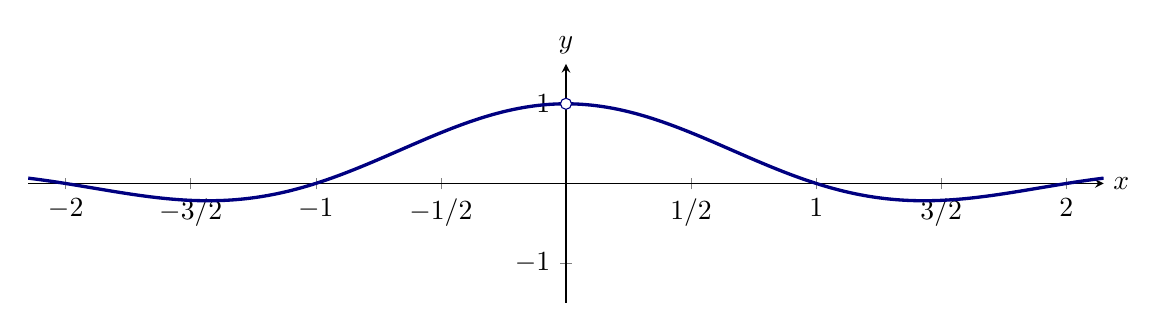
\begin{tikzpicture}
    \begin{axis}[
        xmin=-6.75,xmax=6.75,ymin=-1.5,ymax=1.5,
        axis lines=center,
        xtick={-6.28, -4.71, -3.14, -1.57, 0, 1.57, 3.142, 4.71, 6.28},
        xticklabels={$-2$,$-3/2$,$-1$, $-1/2$, $0$, $1/2$, $1$, $3/2$, $2$},
        ytick={-1,1},
        %ticks=none,
        width=6in,
        height=3in,
        unit vector ratio*=1 1 1,
        xlabel=$x$, ylabel=$y$,
        every axis y label/.style={at=(current axis.above origin),anchor=south},
        every axis x label/.style={at=(current axis.right of origin),anchor=west},
      ]        
      \addplot [very thick, penColor, samples=100,smooth, domain=(-6.75:6.75)] {sin(deg(x))/x};
      
      \addplot[color=penColor,fill=white,only marks,mark=*] coordinates{(0,1)};  %% open hole          
    \end{axis}
  \end{tikzpicture}
\end{image}

\begin{question}
  Use the graph of $f$ above to answer the
  following question: What is $f(0)$?
  \begin{multipleChoice}
    \choice{$0$}
    \choice{$f(0)$}
    \choice{$1$}
    \choice[correct]{$f(0)$ is undefined}
    \choice{it is impossible to say}
  \end{multipleChoice}
\end{question}

Nevertheless, we can see that as $x$ approaches zero, $f(x)$
approaches one. From this setting we come to our definition of a
limit.

\begin{definition}
  Intuitively,
  \begin{center}
    the \dfn{limit} of $f(x)$ as $x$ approaches $a$ is $L$,
  \end{center}
  written
  \[
  \lim_{x\to a} f(x) = L,
  \]
  if the value of $f(x)$ can be made as close as one wishes to $L$ for
  all $x$ sufficiently close, but not equal, to $a$.
\end{definition}

\begin{question}
  Use the graph of $f}$ above to finish the following statement: ``A good guess is that\dots''
  \begin{multipleChoice}
    \choice[correct]{$\lim_{x\to 0}f(x) = 1$.}
    \choice{$\lim_{x\to 1}f(x) = 0$.}
    \choice{$\lim_{x\to 1}f(x) = f(1)$.}
    \choice{$\lim_{x\to 0}f(x) = f(0)$.}
  \end{multipleChoice}
\end{question}


\begin{question}
  Consider the following graph of $y=f(x)$
\begin{image}
          
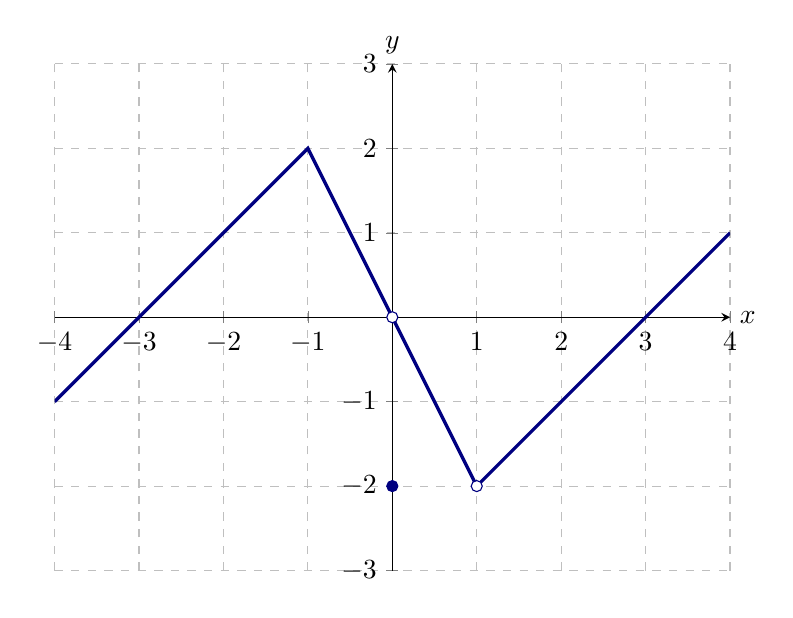
\begin{tikzpicture}
	\begin{axis}[
            xmin=-4, xmax=4, ymin=-3,ymax=3,    
            unit vector ratio*=1 1 1,
            axis lines =middle, xlabel=$x$, ylabel=$y$,
            every axis y label/.style={at=(current axis.above origin),anchor=south},
            every axis x label/.style={at=(current axis.right of origin),anchor=west},
            xtick={-4,...,4}, ytick={-3,...,3},
            %xticklabels={-4,,-2,,0,,2,,4,,6}, yticklabels={,-2,,0,,2,,4,,6,,8,,10},
            grid=major,width=4in,
            grid style={dashed, gridColor},
          ]
	  \addplot[color=penColor,very thick] plot coordinates
                  {(-4,-1) (-1,2) (1,-2) (4,1)};

          \addplot[color=penColor,fill=penColor,only marks,mark=*] coordinates{(0,-2)};  %% closed hole
          \addplot[color=penColor,fill=background,only marks,mark=*] coordinates{(0,0)};  %% open hole
          \addplot[color=penColor,fill=background,only marks,mark=*] coordinates{(1,-2)};  %% open hole
        \end{axis}
\end{tikzpicture}
\end{image}
  Use the graph to evaluate the following. Write DNE if the value does
  not exist.
  \begin{enumerate}
    \item $f(-2) \begin{prompt}=\answer{1}\end{prompt}$
    \item $\lim_{x\to -2}f(x)\begin{prompt}=\answer{1}\end{prompt}$
    \item $f(-1) \begin{prompt}=\answer{2}\end{prompt}$
    \item $\lim_{x\to -1}f(x) \begin{prompt}=\answer{2}\end{prompt}$
    \item $f(0) \begin{prompt}=\answer{-2}\end{prompt}$
    \item $\lim_{x\to 0} f(x) \begin{prompt}=\answer{0}\end{prompt}$
    \item $f(1) \begin{prompt}=\answer{DNE}\end{prompt}$
    \item $\lim_{x\to 1} f(x) \begin{prompt}=\answer{-2}\end{prompt}$
  \end{enumerate}
\end{question}





\section{Limits might not exist}

Limits might not exist. Let's see how this happens.


\begin{example}
  Consider the graph of $f(x) = \lfloor x\rfloor$.
\begin{image}
\begin{tikzpicture}
	\begin{axis}[
            domain=-2:4,
            axis lines =middle, xlabel=$x$, ylabel=$y$,
            every axis y label/.style={at=(current axis.above origin),anchor=south},
            every axis x label/.style={at=(current axis.right of origin),anchor=west},
            clip=false,
          ]
          \addplot [very thick, penColor, domain=(-2:-1)] {-2};
          \addplot [very thick, penColor, domain=(-1:0)] {-1};
          \addplot [very thick, penColor, domain=(0:1)] {0};
          \addplot [very thick, penColor, domain=(1:2)] {1};
          \addplot [very thick, penColor, domain=(2:3)] {2};
          \addplot [very thick, penColor, domain=(3:4)] {3};
          \addplot[color=penColor,fill=penColor,only marks,mark=*] coordinates{(-2,-2)};  %% closed hole          
          \addplot[color=penColor,fill=penColor,only marks,mark=*] coordinates{(-1,-1)};  %% closed hole          
          \addplot[color=penColor,fill=penColor,only marks,mark=*] coordinates{(0,0)};  %% closed hole          
          \addplot[color=penColor,fill=penColor,only marks,mark=*] coordinates{(1,1)};  %% closed hole          
          \addplot[color=penColor,fill=penColor,only marks,mark=*] coordinates{(2,2)};  %% closed hole  
          \addplot[color=penColor,fill=penColor,only marks,mark=*] coordinates{(3,3)};  %% closed hole                  
          \addplot[color=penColor,fill=background,only marks,mark=*] coordinates{(-1,-2)};  %% open hole
          \addplot[color=penColor,fill=background,only marks,mark=*] coordinates{(0,-1)};  %% open hole
          \addplot[color=penColor,fill=background,only marks,mark=*] coordinates{(1,0)};  %% open hole
          \addplot[color=penColor,fill=background,only marks,mark=*] coordinates{(2,1)};  %% open hole
          \addplot[color=penColor,fill=background,only marks,mark=*] coordinates{(3,2)};  %% open hole
          \addplot[color=penColor,fill=background,only marks,mark=*] coordinates{(4,3)};  %% open hole
        \end{axis}
\end{tikzpicture}
%% \caption{A plot of $f(x)=\lfloor x\rfloor$. Note, no matter which
%%   $\delta>0$ is chosen, we can only at best bound $f(x)$ in the
%%   interval $[1,2]$. With the example of $f(x) = \lfloor x \rfloor$, we
%%   see that taking limits is truly different from evaluating
%%   functions.}
\end{image}
Explain why the limit
\[
\lim_{x\to 2} f(x)
\]
does not exist.
\begin{explanation}
The function $\lfloor x \rfloor$ is the function that returns the
greatest integer less than or equal to $x$. Recall that
\[
\lim_{x\to 2} \lfloor x \rfloor  = L
\]
if $\lfloor x\rfloor$ can be made arbitrarily close to $L$ by making
$x$ sufficiently close, but not equal to, $2$. So let's examine $x$
near, but not equal to, $2$. Now the question is: What is $L$?



If this limit exists, then we should be able to look sufficiently
close, but not at, $x=2$, and see that $f$ is approaching some number.
Let's look at a graph:
\begin{image}
\begin{tikzpicture}
	\begin{axis}[
            domain=1.5:2.5,
            ymin=-.5,ymax=3.5,
            axis lines =middle, xlabel=$x$, ylabel=$y$,
            every axis y label/.style={at=(current axis.above origin),anchor=south},
            every axis x label/.style={at=(current axis.right of origin),anchor=west},
          ]
	  \addplot [very thick, penColor, domain=(1:2)] {1};
          \addplot [very thick, penColor, domain=(2:3)] {2};
          \addplot[color=penColor,fill=penColor,only marks,mark=*] coordinates{(2,2)};  %% closed hole  
          \addplot[color=penColor,fill=background,only marks,mark=*] coordinates{(2,1)};  %% open hole
          
          \addplot[(-),color=penColor2,ultra thick] plot coordinates {(1.75,0) (2.25,0)};

          \addplot[color=penColor2,fill=background,only marks,mark=*] coordinates{(2,0)};  %% open hole
          \addplot[textColor,dashed] plot coordinates {(1.9,0) (1.9,1)};
        \end{axis}
\end{tikzpicture}
\end{image}
If we look closer and closer to $x=2$ (on the left of $x=2$) we see
that $f(x) = 1$. However, if we look closer and closer to $x=2$ (on
the right of $x=2$) we see
\begin{image}
\begin{tikzpicture}
	\begin{axis}[
            domain=1.5:2.5,
            ymin=-.5,ymax=3.5,
            axis lines =middle, xlabel=$x$, ylabel=$y$,
            every axis y label/.style={at=(current axis.above origin),anchor=south},
            every axis x label/.style={at=(current axis.right of origin),anchor=west},
          ]
	  \addplot [very thick, penColor, domain=(1:2)] {1};
          \addplot [very thick, penColor, domain=(2:3)] {2};
          \addplot[color=penColor,fill=penColor,only marks,mark=*] coordinates{(2,2)};  %% closed hole  
          \addplot[color=penColor,fill=background,only marks,mark=*] coordinates{(2,1)};  %% open hole
          
          \addplot[(-),color=penColor2,ultra thick] plot coordinates {(1.75,0) (2.25,0)};

          \addplot[color=penColor2,fill=background,only marks,mark=*] coordinates{(2,0)};  %% open hole
          \addplot[textColor,dashed] plot coordinates {(2.1,0) (2.1,2)};
        \end{axis}
\end{tikzpicture}
\end{image}
So just to the right of $x=2$, $f(x)=2$. We cannot find a single
number that $f(x)$ approaches as $x$ approaches $x=2$, and so the
limit does not exists.
\end{explanation}
\end{example}

Tables can be used to help guess limits, but one must be careful.

\begin{question}
  Consider $f(x) = \sin\left(\frac{\pi}{x}\right)$. Fill in the 
  tables below:
  \[
  \begin{array}{l|l}
    x      & f(x)      \\ \hline
    0.1    & \begin{prompt}\answer{0}\end{prompt}\\
    0.01   & \begin{prompt}\answer{0}\end{prompt}\\
    0.001  & \begin{prompt}\answer{0}\end{prompt}\\
    0.0001 & \begin{prompt}\answer{0}\end{prompt} 
  \end{array}
  \qquad\text{and}\qquad
  \begin{array}{l|l}
    x      & f(x)            \\ \hline
    0.3    &  \begin{prompt}\answer{-.866}\end{prompt} \\
    0.03   &  \begin{prompt}\answer{-.866}\end{prompt} \\
    0.003  &  \begin{prompt}\answer{-.866}\end{prompt} \\
    0.0003 &  \begin{prompt}\answer{-.866}\end{prompt}
  \end{array}
  \]
  What do the tables tell us about
  \[
  \lim_{x\to 0}\sin\left(\frac{\pi}{x}\right)?
  \]
  \begin{multipleChoice}
    \choice{$\lim_{x\to 0}\sin\left(\frac{\pi}{x}\right) = 0$}
    \choice{$\lim_{x\to 0}\sin\left(\frac{\pi}{x}\right)=1$}
    \choice{$\lim_{x\to 0}\sin\left(\frac{\pi}{x}\right) = -.866$}
    \choice{$\lim_{x\to 0}\sin\left(\frac{\pi}{x}\right) = -.433$}
    \choice[correct]{it is unclear what the tables are telling us about the limit}
  \end{multipleChoice}
  \begin{feedback}
    Neither tables nor graphs can ever tell us for certain what a
    limit is. However, sometimes they can help ``guess'' the limit. In
    this case the graph of $f(x)$ is somewhat more helpful:
    \begin{image}
      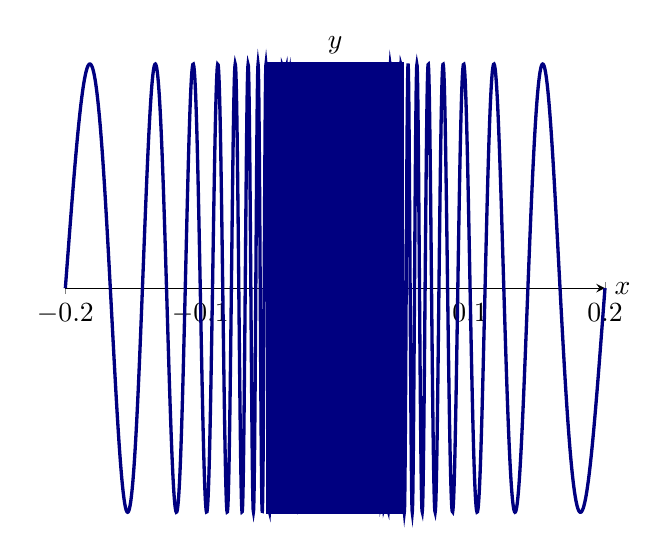
\begin{tikzpicture}
	\begin{axis}[
            domain=-.2:.2,    
            samples=500,
            axis lines =middle, xlabel=$x$, ylabel=$y$,
            yticklabels = {}, 
            every axis y label/.style={at=(current axis.above origin),anchor=south},
            every axis x label/.style={at=(current axis.right of origin),anchor=west},
            clip=false,
          ]
	  \addplot [very thick, penColor, smooth, domain=(-.2:-.02)] {sin(deg(pi/x))};
          \addplot [very thick, penColor, smooth, domain=(.02:.2)] {sin(deg(pi/x))};
	  \addplot [color=penColor, fill=penColor, very thick, smooth,domain=(-.05:.05)] {1} \closedcycle;
          \addplot [color=penColor, fill=penColor, very thick, smooth,domain=(-.05:.05)] {-1} \closedcycle;
        \end{axis}
      \end{tikzpicture}
    \end{image}
   We see that $f(x)$ oscillates ``wildly'' as $x$ approaches $0$, and hence does not approach any one number.
  \end{feedback}
\end{question}



\section{One-sided limits}


While we have seen that $\lim_{x\to 2}\lfloor x\rfloor$ does not
exist, more can still be said.



\begin{definition}
  Intuitively,
  \begin{center}
    the \dfn{limit from the right} of $f$ as $x$ approaches $a$ is
    $L$,
  \end{center}
  written
  \[
  \lim_{x\to a^+} f(x) = L,
  \]
  if the value of $f(x)$ can be made as close as one wishes to $L$ for
  all $x>a$ sufficiently close, but not equal to, $a$.
  
  Similarly,
  \begin{center}
    the \dfn{limit from the left} of $f(x)$ as $x$ approaches $a$ is
    $L$,
  \end{center}
  written
  \[
  \lim_{x\to a^-} f(x) = L,
  \]
  if the value of $f(x)$ can be made as close as one wishes to $L$ for
  all $x<a$ sufficiently close, but not equal to, $a$.
\end{definition}


\begin{example}
Compute:
\[
\lim_{x\to 2^-} f(x)\qquad\text{and}\qquad \lim_{x\to 2^+} f(x)
\]
by using the graph below
\begin{image}
\begin{tikzpicture}
	\begin{axis}[
            domain=-2:4,
            axis lines =middle, xlabel=$x$, ylabel=$y$,
            every axis y label/.style={at=(current axis.above origin),anchor=south},
            every axis x label/.style={at=(current axis.right of origin),anchor=west},
            clip=false,
          ]
          \addplot [very thick, penColor, domain=(-2:-1)] {-2};
          \addplot [very thick, penColor, domain=(-1:0)] {-1};
          \addplot [very thick, penColor, domain=(0:1)] {0};
          \addplot [very thick, penColor, domain=(1:2)] {1};
          \addplot [very thick, penColor, domain=(2:3)] {2};
          \addplot [very thick, penColor, domain=(3:4)] {3};
          \addplot[color=penColor,fill=penColor,only marks,mark=*] coordinates{(-2,-2)};  %% closed hole          
          \addplot[color=penColor,fill=penColor,only marks,mark=*] coordinates{(-1,-1)};  %% closed hole          
          \addplot[color=penColor,fill=penColor,only marks,mark=*] coordinates{(0,0)};  %% closed hole          
          \addplot[color=penColor,fill=penColor,only marks,mark=*] coordinates{(1,1)};  %% closed hole          
          \addplot[color=penColor,fill=penColor,only marks,mark=*] coordinates{(2,2)};  %% closed hole  
          \addplot[color=penColor,fill=penColor,only marks,mark=*] coordinates{(3,3)};  %% closed hole                  
          \addplot[color=penColor,fill=background,only marks,mark=*] coordinates{(-1,-2)};  %% open hole
          \addplot[color=penColor,fill=background,only marks,mark=*] coordinates{(0,-1)};  %% open hole
          \addplot[color=penColor,fill=background,only marks,mark=*] coordinates{(1,0)};  %% open hole
          \addplot[color=penColor,fill=background,only marks,mark=*] coordinates{(2,1)};  %% open hole
          \addplot[color=penColor,fill=background,only marks,mark=*] coordinates{(3,2)};  %% open hole
          \addplot[color=penColor,fill=background,only marks,mark=*] coordinates{(4,3)};  %% open hole
        \end{axis}
\end{tikzpicture}
%% \caption{A plot of $f(x)=\lfloor x\rfloor$. Note, no matter which
%%   $\delta>0$ is chosen, we can only at best bound $f(x)$ in the
%%   interval $[1,2]$. With the example of $f(x) = \lfloor x \rfloor$, we
%%   see that taking limits is truly different from evaluating
%%   functions.}
\end{image}
\begin{explanation}
  From the graph we can see that as $x$ approaches $2$ from the left, $\lfloor x\rfloor$ remains at $y=1$ up  until the exact point that $x=2$. Hence
  \[
  \lim_{x\to 2^-} f(x)=1.
  \]
  Also from the graph we can see that as $x$ approaches $2$ from the
  right, $\lfloor x\rfloor$ remains at $y=2$ up to $x=2$. Hence
  \[
  \lim_{x\to 2^+} f(x)=2.
  \]
\end{explanation}
\end{example}



\section{When you put this all together}

One-sided limits help us talk about limits.
\begin{theorem}\index{limit}\index{one-sided limit}
  A limit
  \[
  \lim_{x \to a} f(x)
  \]
  exists if and only if
  \begin{itemize}
  \item $\lim_{x \to a^-} f(x)$ exists
  \item $\lim_{x \to a^+} f(x)$ exists
  \item $\lim_{x \to a^-} f(x) = \lim_{x \to a^+} f(x)$
  \end{itemize}
  In this case, $\lim_{x \to a} f(x)$ is equal to the common
  value of the two one sided limits.
\end{theorem}


\begin{question}
  Evaluate the expressions by referencing the graph below. Write DNE
  if the limit does not exist.
\begin{image}
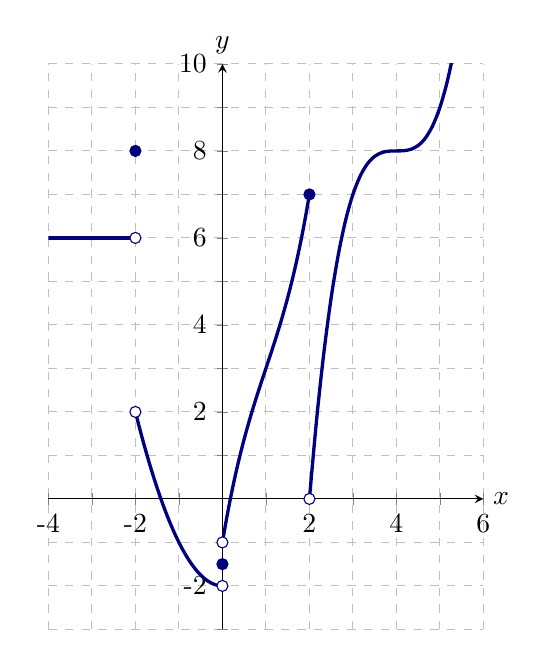
\begin{tikzpicture}
	\begin{axis}[
            domain=-4:6, xmin=-4, xmax=6, ymin=-3,ymax=10,    
            unit vector ratio*=1 1 1,
            axis lines =middle, xlabel=$x$, ylabel=$y$,
            every axis y label/.style={at=(current axis.above origin),anchor=south},
            every axis x label/.style={at=(current axis.right of origin),anchor=west},
            xtick={-4,...,6}, ytick={-3,...,10},
            xticklabels={-4,,-2,,0,,2,,4,,6}, yticklabels={,-2,,0,,2,,4,,6,,8,,10},
            grid=major,width=4in,
            grid style={dashed, gridColor},
          ]
	  \addplot [very thick, penColor, smooth, domain=(-4:-2)] {6};
	  \addplot [very thick, penColor, smooth, domain=(-2:0)] {x^2-2};
          \addplot [very thick, penColor, smooth, domain=(0:2)] {(x-1)^3+3*(x-1)+3};
          \addplot [very thick, penColor, smooth, domain=(2:6)] {(x-4)^3+8};
          \addplot[color=penColor,fill=background,only marks,mark=*] coordinates{(-2,6)};  %% open hole
          \addplot[color=penColor,fill=background,only marks,mark=*] coordinates{(-2,2)};  %% open hole
          \addplot[color=penColor,fill=background,only marks,mark=*] coordinates{(0,-2)};  %% open hole
          \addplot[color=penColor,fill=background,only marks,mark=*] coordinates{(0,-1)};  %% open hole
          \addplot[color=penColor,fill=background,only marks,mark=*] coordinates{(2,0)};  %% open hole
          \addplot[color=penColor,fill=penColor,only marks,mark=*] coordinates{(-2,8)};  %% closed hole
          \addplot[color=penColor,fill=penColor,only marks,mark=*] coordinates{(0,-1.5)};  %% closed hole
          \addplot[color=penColor,fill=penColor,only marks,mark=*] coordinates{(2,7)};  %% closed hole
        \end{axis}
\end{tikzpicture}
\end{image}
\begin{enumerate}
\item $\lim_{x\to 4} f(x) \begin{prompt}=\answer{8}\end{prompt}$  
\item $\lim_{x\to -3} f(x)\begin{prompt}=\answer{6}\end{prompt}$  
\item $\lim_{x\to 0} f(x) \begin{prompt}=\answer{DNE}\end{prompt}$ 
\item $\lim_{x\to 0^-} f(x) \begin{prompt}=\answer{-2}\end{prompt}$  
\item $\lim_{x\to 0^+} f(x) \begin{prompt}=\answer{-1}\end{prompt}$  
\item $f(-2) \begin{prompt}=\answer{8}\end{prompt}$  
\item $\lim_{x\to 2^-} f(x) \begin{prompt}=\answer{7}\end{prompt}$  
\item $\lim_{x\to -2^-} f(x) \begin{prompt}=\answer{6}\end{prompt}$  
\item $\lim_{x\to 0} f(x+1) \begin{prompt}=\answer{3}\end{prompt}$  
\item $f(0) \begin{prompt}=\answer{-3/2}\end{prompt}$ 
\item $\lim_{x\to 1^-} f(x-4) \begin{prompt}=\answer{6}\end{prompt}$  
\item $\lim_{x\to 0^+} f(x-2) \begin{prompt}=\answer{2}\end{prompt}$
\end{enumerate}
\end{question}



\end{document}
